%% aframe_subprocess_comm.tex  –  Subprocess communication swimlane diagram
%% Compile:  pdflatex aframe_subprocess_comm.tex && pdfcrop aframe_subprocess_comm.pdf
\documentclass{article}
\usepackage[margin=1cm, paperwidth=38cm, paperheight=17cm]{geometry}
\pagestyle{empty}
\usepackage{tikz}
\usetikzlibrary{positioning,arrows.meta,fit,backgrounds,calc}

\colorlet{mainfill}{blue!10}   \colorlet{mainbrd}{blue!55!black}
\colorlet{subfill} {orange!12} \colorlet{subbrd} {orange!65!black}
\colorlet{qfill}   {teal!10}   \colorlet{qbrd}   {teal!55!black}
\colorlet{extfill} {purple!12} \colorlet{extbrd} {purple!55!black}
\colorlet{memfill} {green!8}   \colorlet{membrd} {green!50!black}

\begin{document}
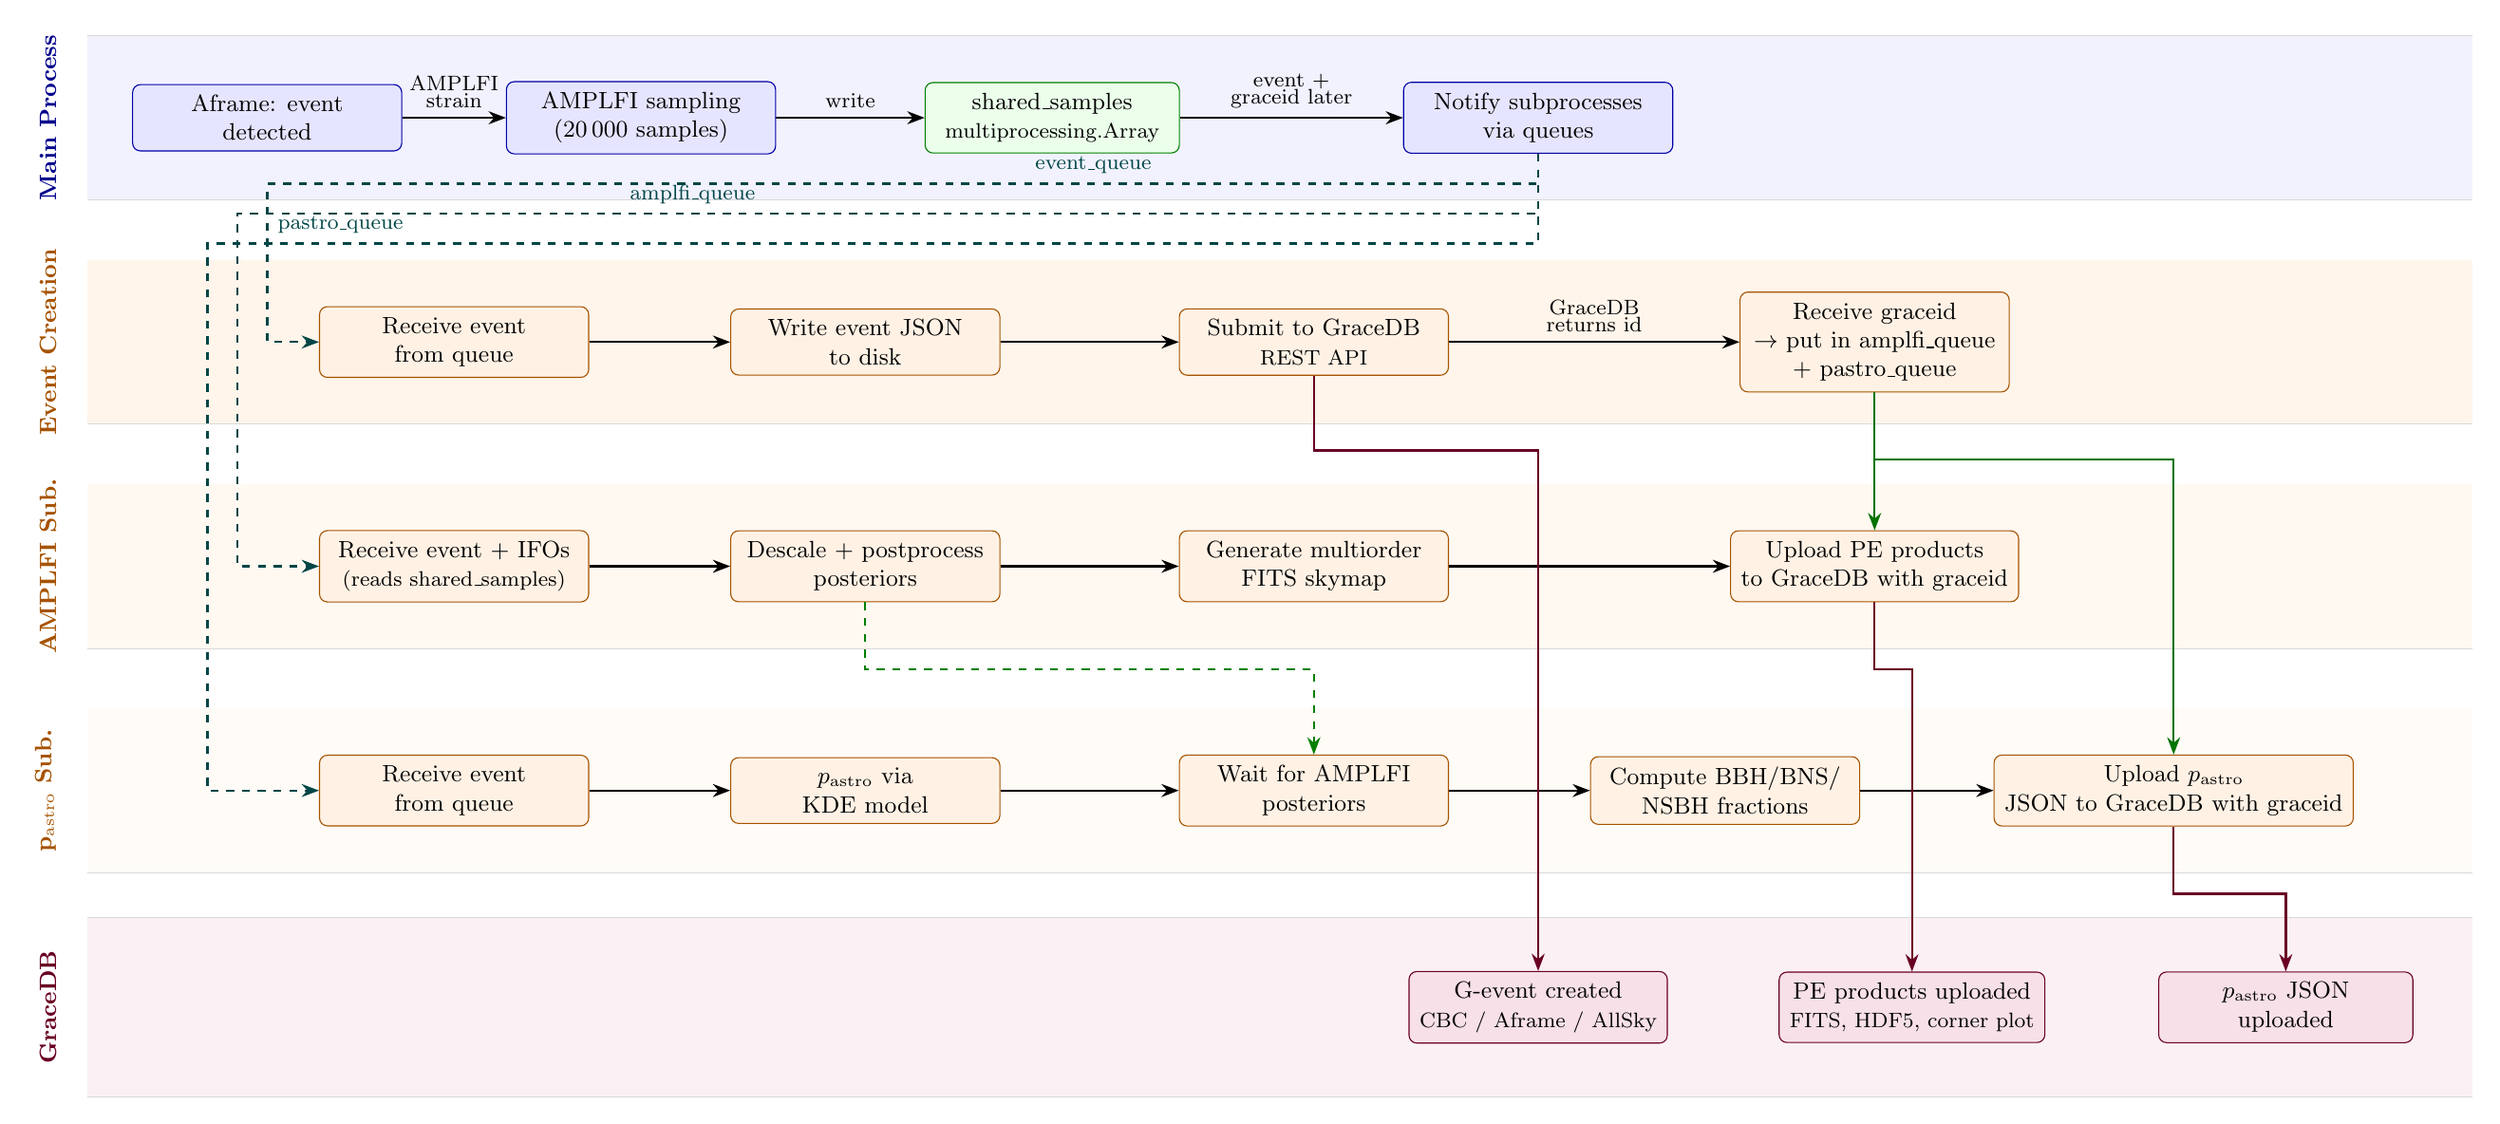
\begin{tikzpicture}[
  >=Stealth,
  every node/.style={font=\small, align=center},
  step/.style  ={draw=#1!65!black, fill=#1!10, rounded corners=3pt,
                 minimum width=3.6cm, minimum height=0.75cm, inner sep=4pt},
  step/.default=blue,
  shmem/.style ={draw=membrd, fill=memfill, rounded corners=3pt,
                 minimum width=3.4cm, minimum height=0.75cm, inner sep=4pt},
  upload/.style={draw=extbrd, fill=extfill, rounded corners=3pt,
                 minimum width=3.4cm, minimum height=0.75cm, inner sep=4pt},
  arr/.style   ={->, thick},
  qarr/.style  ={->, thick, dashed, qbrd},
  garr/.style  ={->, thick, extbrd},
  grdarr/.style={->, thick, green!45!black},
  lane/.style  ={font=\small\bfseries, rotate=90, anchor=south},
]

%% ── Swimlane boundaries ───────────────────────────────────────────────────
%% Main Process:       y = 9.5 – 11.5
%% Event Creation:     y = 6.5 –  8.5
%% AMPLFI Sub:         y = 3.5 –  5.5
%% P_astro Sub:        y = 0.5 –  2.5
%% GraceDB:            y = -2.5 – -0.5

\begin{pgfonlayer}{background}
  \fill[blue!5]    (-0.4, 9.3)  rectangle (31.5, 11.5);
  \fill[orange!8]  (-0.4, 6.3)  rectangle (31.5,  8.5);
  \fill[orange!5]  (-0.4, 3.3)  rectangle (31.5,  5.5);
  \fill[orange!3]  (-0.4, 0.3)  rectangle (31.5,  2.5);
  \fill[purple!6]  (-0.4,-2.7)  rectangle (31.5, -0.3);
  \foreach \y in {9.3, 6.3, 3.3, 0.3, -0.3, -2.7}
    \draw[gray!30, thin] (-0.4,\y) -- (31.5,\y);
  \draw[gray!30, thin] (-0.4,11.5) -- (31.5,11.5);
\end{pgfonlayer}

\node[lane, mainbrd] at (-0.7, 10.4) {Main Process};
\node[lane, subbrd]  at (-0.7,  7.4) {Event Creation};
\node[lane, subbrd]  at (-0.7,  4.4) {AMPLFI Sub.};
\node[lane, subbrd]  at (-0.7,  1.4) {p$_{\mathrm{astro}}$ Sub.};
\node[lane, extbrd]  at (-0.7, -1.5) {GraceDB};

%% ════════════════════════════════════════════════════════════
%% MAIN PROCESS ROW  y = 10.4
%% ════════════════════════════════════════════════════════════
\node[step=blue] (detect) at (2.0, 10.4)
  {Aframe: event\\detected};
\node[step=blue] (amplfi_run) at (7.0, 10.4)
  {AMPLFI sampling\\(20\,000 samples)};
\node[shmem] (shared) at (12.5, 10.4)
  {shared\_samples\\{\footnotesize multiprocessing.Array}};
\node[step=blue] (put_q) at (19.0, 10.4)
  {Notify subprocesses\\via queues};

\draw[arr] (detect)     -- node[above,font=\footnotesize]{AMPLFI\\[-3pt]strain} (amplfi_run);
\draw[arr] (amplfi_run) -- node[above,font=\footnotesize]{write} (shared);
\draw[arr] (shared)     -- node[above,font=\footnotesize]{event +\\[-3pt]graceid later} (put_q);

%% ════════════════════════════════════════════════════════════
%% EVENT CREATION ROW  y = 7.4
%% ════════════════════════════════════════════════════════════
\node[step=orange] (ev_recv)  at (4.5,  7.4) {Receive event\\from queue};
\node[step=orange] (ev_write) at (10.0, 7.4) {Write event JSON\\to disk};
\node[step=orange] (ev_sub)   at (16.0, 7.4) {Submit to GraceDB\\{\footnotesize REST API}};
\node[step=orange] (ev_gid)   at (23.5, 7.4) {Receive graceid\\$\to$ put in amplfi\_queue\\+ pastro\_queue};

\draw[arr] (ev_recv)  -- (ev_write);
\draw[arr] (ev_write) -- (ev_sub);
\draw[arr] (ev_sub)   -- node[above,font=\footnotesize]{GraceDB\\[-3pt]returns id} (ev_gid);

%% ════════════════════════════════════════════════════════════
%% AMPLFI SUB ROW  y = 4.4
%% ════════════════════════════════════════════════════════════
\node[step=orange] (amp_recv) at (4.5,  4.4)
  {Receive event + IFOs\\{\footnotesize (reads shared\_samples)}};
\node[step=orange] (amp_post) at (10.0, 4.4) {Descale + postprocess\\posteriors};
\node[step=orange] (amp_sky)  at (16.0, 4.4) {Generate multiorder\\FITS skymap};
\node[step=orange] (amp_up)   at (23.5, 4.4) {Upload PE products\\to GraceDB with graceid};

\draw[arr] (amp_recv) -- (amp_post);
\draw[arr] (amp_post) -- (amp_sky);
\draw[arr] (amp_sky)  -- (amp_up);

%% ════════════════════════════════════════════════════════════
%% P_ASTRO SUB ROW  y = 1.4
%% ════════════════════════════════════════════════════════════
\node[step=orange] (pa_recv) at (4.5,  1.4) {Receive event\\from queue};
\node[step=orange] (pa_kde)  at (10.0, 1.4) {$p_{\mathrm{astro}}$ via\\KDE model};
\node[step=orange] (pa_post) at (16.0, 1.4) {Wait for AMPLFI\\posteriors};
\node[step=orange] (pa_frac) at (21.5, 1.4) {Compute BBH/BNS/\\NSBH fractions};
\node[step=orange] (pa_up)   at (27.5, 1.4) {Upload $p_{\mathrm{astro}}$\\JSON to GraceDB with graceid};

\draw[arr] (pa_recv) -- (pa_kde);
\draw[arr] (pa_kde)  -- (pa_post);
\draw[arr] (pa_post) -- (pa_frac);
\draw[arr] (pa_frac) -- (pa_up);

%% ════════════════════════════════════════════════════════════
%% GRACEDB ROW  y = -1.5
%% ════════════════════════════════════════════════════════════
\node[upload] (gdb_ev) at (19.0,-1.5) {G-event created\\{\footnotesize CBC / Aframe / AllSky}};
\node[upload] (gdb_pe) at (24.0,-1.5) {PE products uploaded\\{\footnotesize FITS, HDF5, corner plot}};
\node[upload] (gdb_pa) at (29.0,-1.5) {$p_{\mathrm{astro}}$ JSON\\uploaded};

%% ════════════════════════════════════════════════════════════
%% CROSS-LANE ARROWS
%% ════════════════════════════════════════════════════════════

%% put_q → queues → subprocesses  (labels on the long westward segment, spread out)
\draw[qarr]
  (put_q.south) -- ++(0,-0.4)
  -- node[pos=0.35,  above, font=\footnotesize]{event\_queue}   ++(-17,0)
  |- (ev_recv.west);

\draw[qarr]
  (put_q.south) -- ++(0,-0.8)
  -- node[pos=0.65,  above, font=\footnotesize]{amplfi\_queue}  ++(-17.4,0)
  |- (amp_recv.west);

\draw[qarr]
  (put_q.south) -- ++(0,-1.2)
  -- node[pos=0.9,  above, font=\footnotesize]{pastro\_queue}  ++(-17.8,0)
  |- (pa_recv.west);

%% Event Creation submits to GraceDB
\draw[garr] (ev_sub.south) -- ++ (0, -1.0) -| (gdb_ev.north);

%% graceid from ev_gid → amp_up and pa_frac
\draw[grdarr]
  (ev_gid.south) -- ++(0,-1.2) -| (amp_up.north);
\draw[grdarr]
  (ev_gid.south) -- ++(0,-0.9)
  -| (pa_up.north);

%% AMPLFI uploads PE products
\draw[garr]
  (amp_up.south) -- ++(0,-0.9) -| (gdb_pe.north);

%% P_astro uploads p_astro
\draw[garr]
  (pa_up.south) -- ++(0,-0.9) -| (gdb_pa.north);

%% Posterior HDF5 dependency: AMPLFI → P_astro (pa_post waits for it)
\draw[->, thick, membrd, dashed]
  (amp_post.south) -- ++(0,-0.9) -| (pa_post.north);

\end{tikzpicture}
\end{document}
